
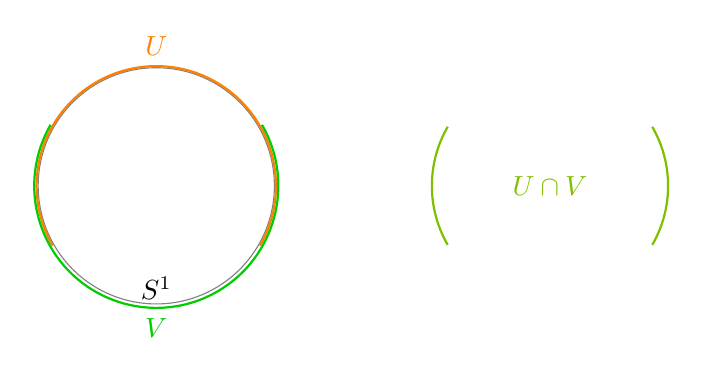
\begin{tikzpicture}
\begin{scope}
\draw[thin, gray] (0,0) circle [radius = 1.5cm];
\node at (0, -1.3) {$\mathbb{S}^1$};

\draw[thick, orange] ({1.52 * cos(-30)}, {1.52 * sin(-30)}) arc (-30:210:1.52cm) node[midway, above] {$U$};
\draw[thick, green!80!black] ({1.55 * cos(30)}, {1.55 * sin(30)}) arc (30:-210:1.55cm) node[midway, below] {$V$};
\end{scope}

\begin{scope}[xshift = 5cm]
\draw[thick, orange!50!green] ({1.5 * cos(30)}, {1.5 * sin(30)}) arc (30:-30:1.5cm);
\draw[thick, orange!50!green] ({1.5 * cos(150)}, {1.5 * sin(150)}) arc (150:210:1.5cm);
\node[orange!50!green] at (0,0) {$U \cap V$};
\end{scope}
\end{tikzpicture}
